\documentclass[]{article}
\usepackage{graphicx}
\usepackage{hyperref}
\usepackage{float}
\usepackage[a4paper,bindingoffset=0.2in,%
            left=0.75in,right=0.75in,top=1in,bottom=1in,%
            footskip=.25in]{geometry}

%opening
\title{Assignment 2 CDA}
\author{Tim van Rossum, 4246306\\
	Michiel Doesburg, 4343875}

\begin{document}

\maketitle
\section{Familiarization with the data}
The dataset contains a total of 44 signals, with some being static values, other being sinusoid signals, and others being partially discrete (as in, they can rise or drop at certain points). L-signals tend to be more sinusoidal, F-signals tend to be "partially discrete", and S-signals are all binary signals.

All the signals together seem to have little correlation. Some combinations of signals are reasonably correlated: e.g. L\_T3 and P\_J302 have a 0.42 correlation coefficient. Moreover, the signal P\_J302 in figure 3 looks cyclic. A cyclic signal like this is much easier to predict than a `random' signal, since there is a rough base model that it adheres to. This signal's values are within a clear band at about 2-6 on the Y-axis. In such a case it is very easy to come up with a basic anomaly detection technique: if the signal moves outside this band this would be a clear sign of an anomaly. Plotting the mean error we saw for the ARMA prediction on signal L\_T1, we saw that there were only 2 cases were the error was greater than three times the standard deviation. 

\begin{center}
\begin{figure}[H]
\begin{minipage}{.475\textwidth}
  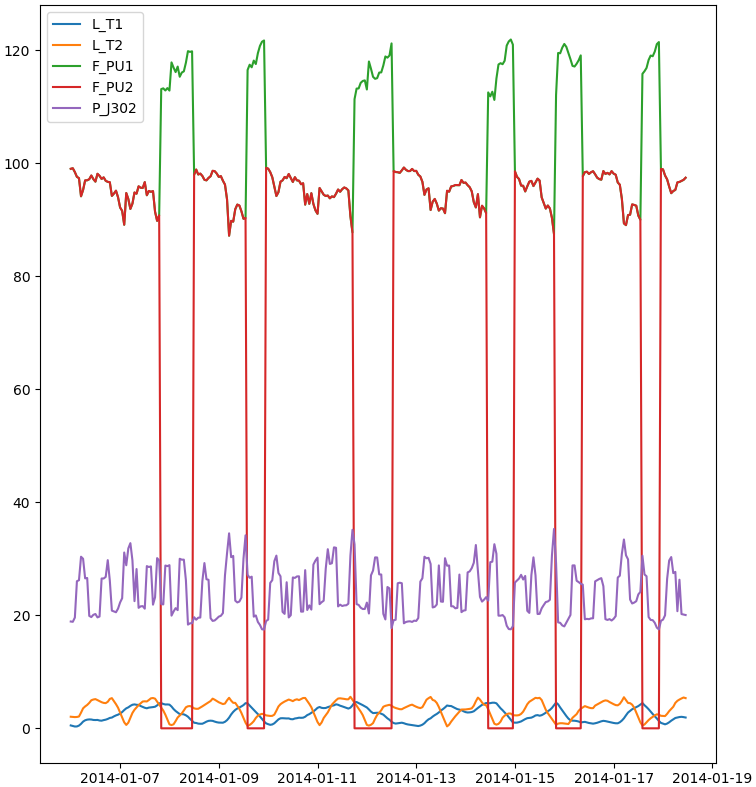
\includegraphics[width=1\linewidth, height=4.5cm]{./visuallizations/signals.png}
  \caption{Visualization of some signals. The red and green signals are partially discrete.}
  \label{signals}
\end{minipage} %
\begin{minipage}{.475\textwidth}
  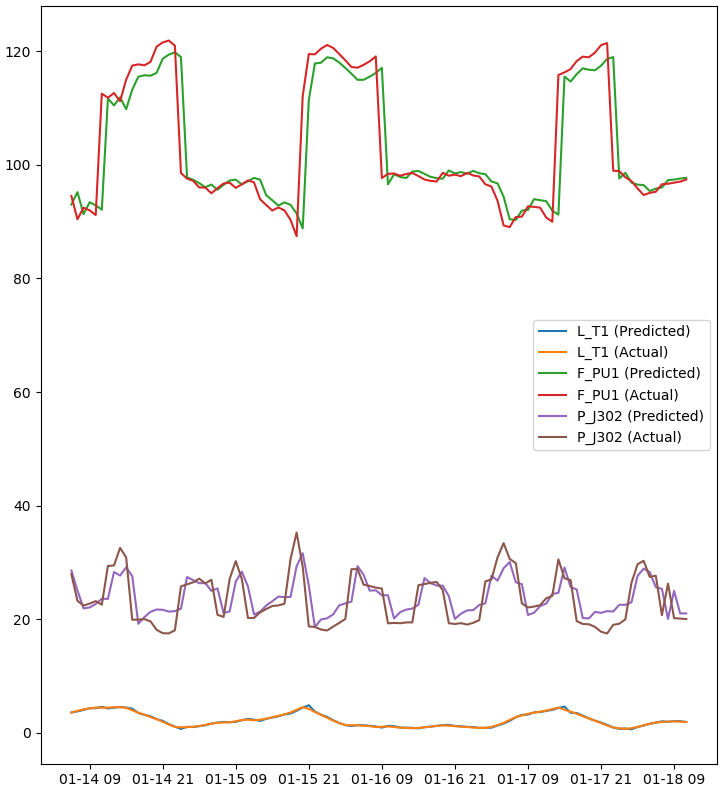
\includegraphics[width=1\linewidth, height=4.5cm]{./visuallizations/predictions.png}
   \caption{ARMA predictions on some signals. The predictions work better on signals with fewer rapid changes.}
  \label{predictions}
\end{minipage}
\begin{minipage}{\textwidth}
  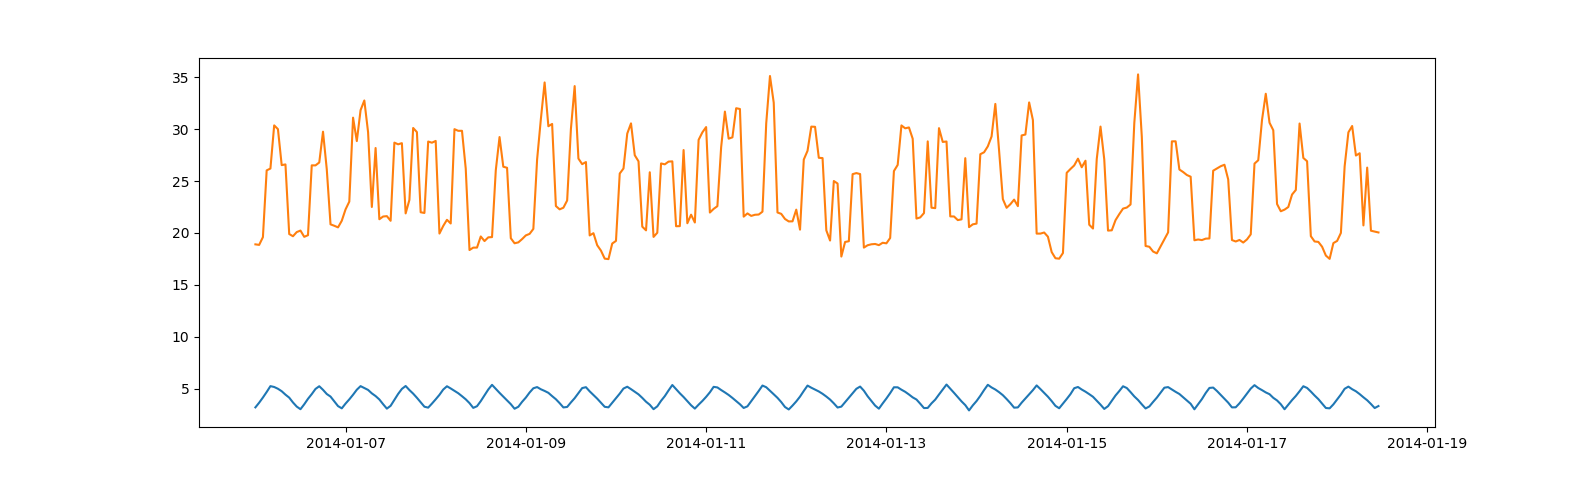
\includegraphics[width=1\linewidth, height=4cm]{./visuallizations/correlated_signals.png}.
  \label{correlation}
  \caption{Signals L\_T3 and P\_J302. The peaks are roughly aligned. These signals have around 40\% correlation.}
\end{minipage}%
\end{figure}
\end{center}

\clearpage
\section{ARMA}
The script \texttt{ARMA.py} learns a ARMA model for any particular sensor. The parameters for the model are determined by testing out different $p$'s and $q$'s on the training data and then looking at the AIC value of the fitted model. A lower AIC means a better fit. Fitting the models takes quite some time, and as such the search space for parameters is limited. For $p$, only values in the range of $[0, 4]$ are tested, and for $q$, only values in the range of $[0, 2]$ are tested. Both these ranges are inclusive. We thought these ranges would still allow for a reasonable search space while limiting the time taken to search for the ideal parameters. Predictions are then done on the test data, with the exception of the first 30 values in the signal, as these are used as initial values for ARMA to base predictions on.

After the predictions are done, the predicted values are compared to the actual values. The difference between the two is used, and then the mean of the absolute values is computed, along with the standard deviation of the absolute values. An attack is detected if a predicted value differs from the actual value by more than the threshold, which is given by the absolute mean plus a number of times the standard deviation. We used mean absolute error instead of root mean squared error because the root mean squared error gives a larger weight to larger errors. The sensors that have cyclic time series can be modelled effectively by ARMA, and the anomalies that can be detected are contextual anomalies. Sensors that have rapid changes are less effectively modeled by ARMA, what can usually be seen is that the prediction lags behind the actual values, like in figure 2. 
\begin{center}
\begin{figure}[H]
  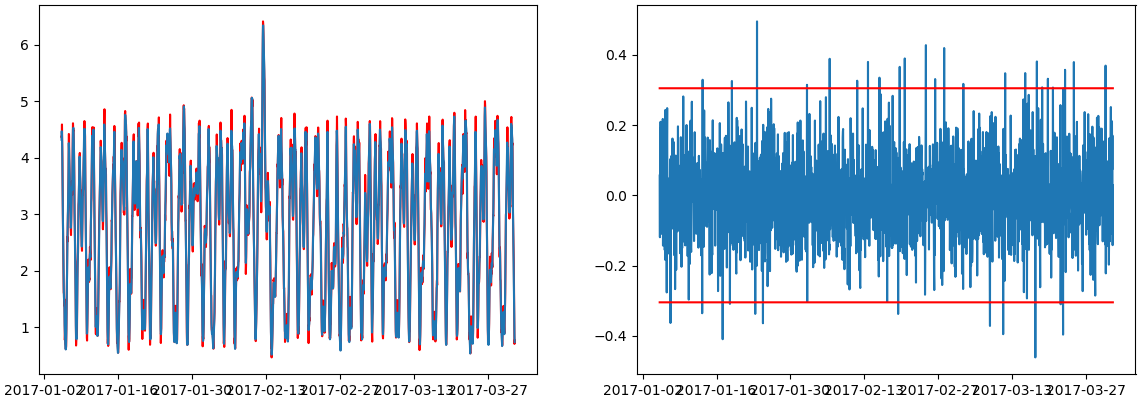
\includegraphics[width=16cm, height=3cm]{./visuallizations/arma_3stddev_LTU1.png}
  \caption{The prediction for signal L\_TU1. On the left is the signal in blue versus the predicted signal in red. On the right are the residual errors and the threshold.}
  \label{signals}
\end{figure}
\end{center}
% We can use this for the comparison part.
% When setting the threshold to 3 times the standard deviation we can see that there are a lot of detected anomalies. Looking at the signal, most of these are probably benign. The threshold might need to be set a little higher for this signal to weed out a few more (likely) false positives.
\section{Discrete models}
For this task, we used the SAX method as shown in class. The script \texttt{SAX.py} is a script that can discretize a time series using SAX. The script was provided by Qin Lin, and we altered a few things to make it work with Python 3. Discretization of the signal in this way creates a representative string of characters of the signal, which allows us to perform sequential data mining methods on it. This is in contrast to PAA, which only discretizes the signal, which does not allow us to perform these data mining methods. Discretization by use of SAX makes sense as the signal values are now grouped by how much they differ from the mean of the signal. The window size determines how many mean values the signal will be converted to, and the amount of original data points used per mean. Using a very large window size will obviously result in a very rough approximation and much data loss, using a very small window size will simply approach the original data and be pointless. After some trial-and-error, we found a window size of 3 to work well. The alphabet size determines the range of possible discrete values the means will be mapped to. We did experiment with setting the alphabet size to different values, but this caused us to miss obvious anomalies that we detected earlier, so we just used the standard value of 7.

The script \texttt{applying\_SAX.py} does not only apply SAX on the signals, but also applies the N-grams data mining method to find anomalies. An N-gram is anomalous (and possibly an indicator of an attack) if the score is lower than or equal to either the mean score minus three times the standard deviation, or the minimum score, whichever is higher. The minimum scores was chosen to prevent the score boundary from becoming negative. It is rather rare to have that happen on this data though, as having large word sizes allows us to have a mean score of around 0.98 for most signals with a standard deviation of about 0.2. The sensors that do not have cyclic time series can be modelled effectively by SAX, and the anomalies that can be detected are collective anomalies, as can be seen in the visualization in figure 5.
\clearpage
\section{PCA}
For this task, we first transformed the dataset using PCA. We do not normalize the signals as some signals have a standard deviation of 0. This does have the side effect that the first principal component will dominate the calculation of the residuals. We use 30 principal components, as through trial-and-error testing we found that this amount very clearly distinguishes normal data from possibly anomalous data. The procedure can be found in the script \texttt{PCA.py}. We used the PCA implementation in Scikit-learn because we use Python as our platform. After the dataset was transformed, we performed anomaly detection as described by Lakhina, Crovella and Diot\cite{lakhina2004diagnosing}. The code adheres as much as possible to the variable names used in the paper. A timestamp contains an attack if the squared prediction error is higher than the mean squared prediction error plus three times the standard deviation, or lower than the mean minus three times the standard deviation. A plot of the squared prediction error and the lower and upper bounds for anomalous behaviour is shown in figure 6. Using this method, we can detect point anomalies. In total we detected 19 point anomalies in 3 anomalous regions. On manual inspection many of the point anomalies corresponded to at least one signal which did in fact have a suspicious deviation from its usual behaviour at the same point, and as such were correctly labeled as anomalous. Since only 19 anomalies were detected, there is also not an overflow of false positives present. So PCA seems to strike a nice balance between finding true positives while keeping false positives low.
 
\begin{center}
	\begin{figure}[H]
		\begin{minipage}{.475\textwidth}
			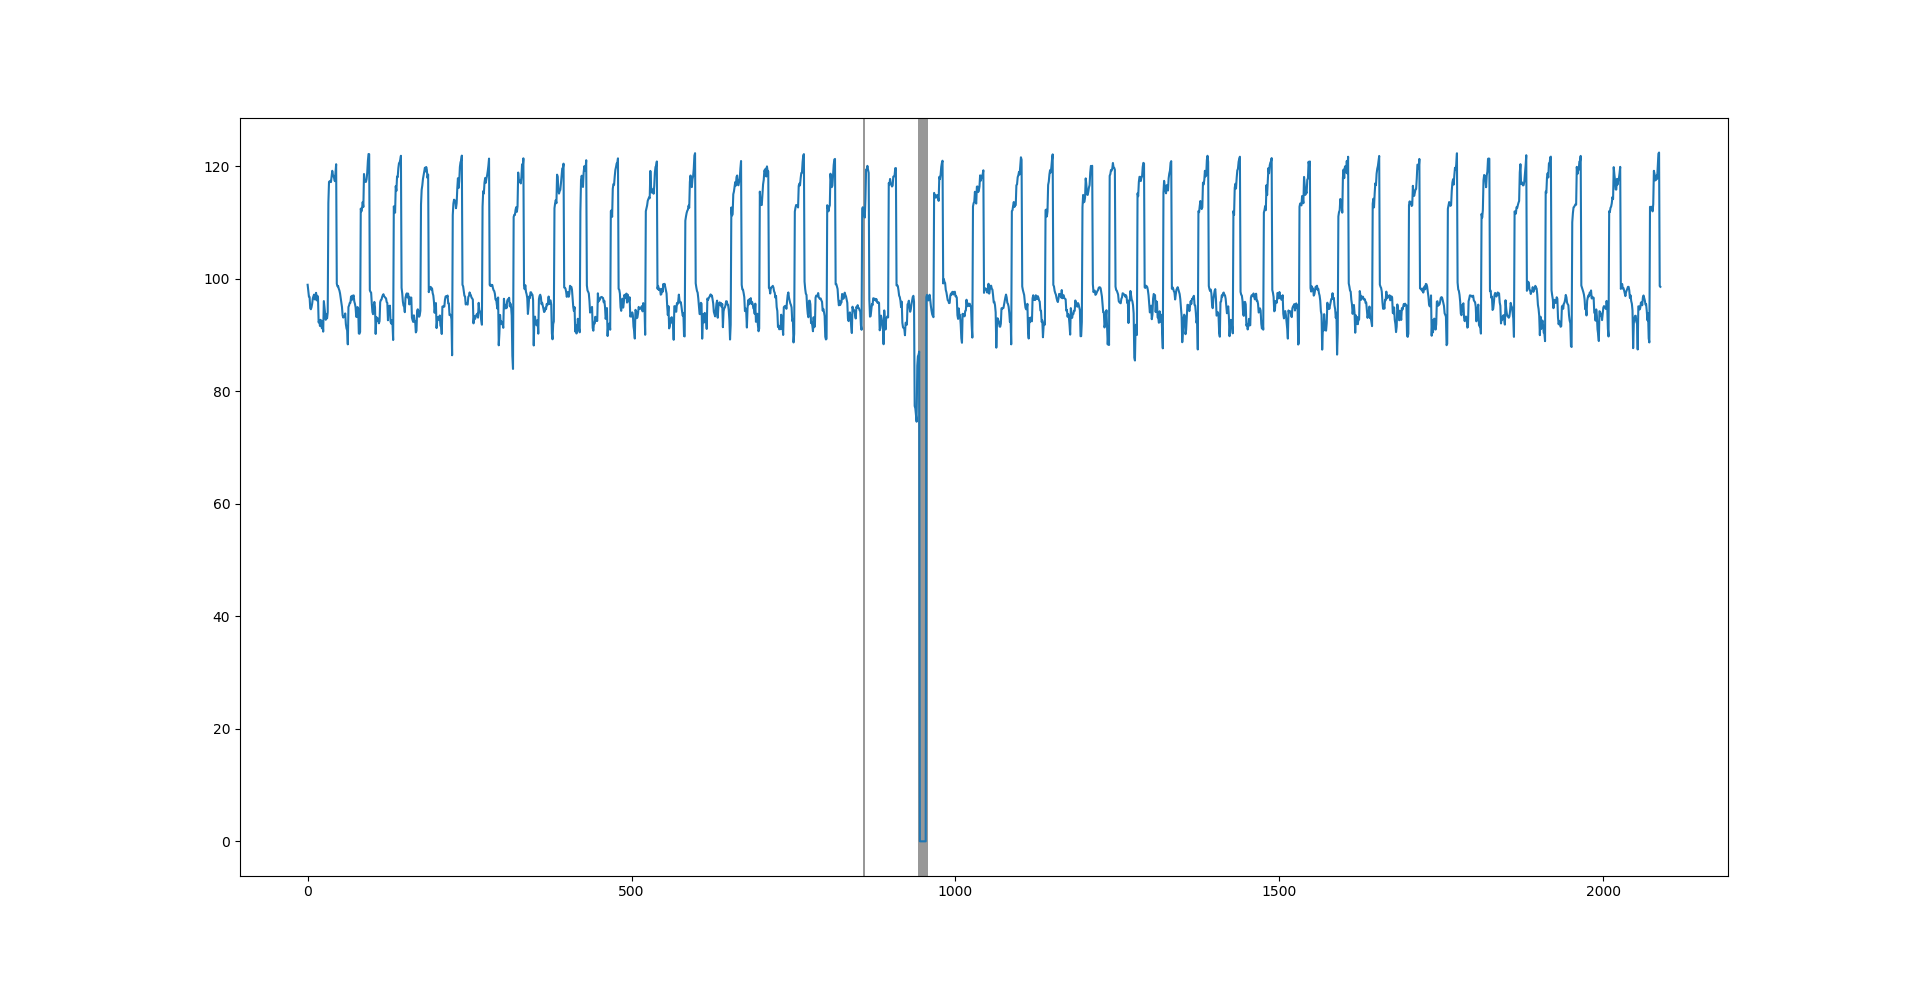
\includegraphics[width=1\linewidth, height=4.5cm]{./visuallizations/SAX_anomaly.png}
			\caption{SAX and Ngrams applied to signal F\_PU1. The anomalous regions are highlighted in yellow.}
			\label{predictions}
		\end{minipage}
		\begin{minipage}{.475\textwidth}
			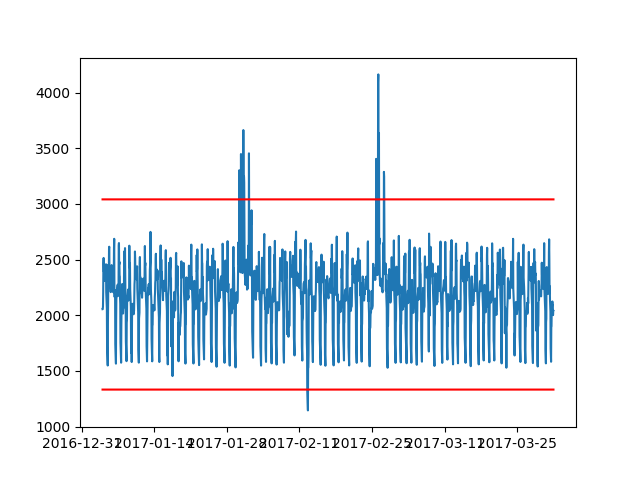
\includegraphics[width=1\linewidth, height=4.5cm]{./visuallizations/PCA_residuals.png}
			\caption{The PCA residuals plotted as the squared prediction error. There are 3 clear anomalous regions.}
			\label{PCA}
		\end{minipage} %
	\end{figure}
\end{center}
\clearpage
\section{Comparison}
Comparing the detection methods will be done as follows: the days on which an anomaly was detected by the PCA method will be used as a base to compare other methods with. Then, the other methods will be executed on all signals that are applicable to those methods, and we will count the amount of overlapping dates on which anomalies were detected. Overlapping dates will count as true positives while non-overlapping dates will count as false positives. The PCA method was chosen as base because this method can be used to detect anomalies in all signals at once, whereas the other two methods can only be used to detect anomalies in one signal at a time. We will also use the other methods to check if PCA does not miss some anomalies that can be observed quite clearly to be actual anomalies (such as the one in figure 5), as well as check how many of the PCA-detected dates were detected at least once to contain an anomaly by the other two methods. These last two are meant to cross validate detected anomalies across methods. The results are shown in table 1.
\begin{table}[h!]
	\centering
	\begin{tabular}{|c|c|c|c|c|}
		\hline
		Method         & True positives & False positives & \begin{tabular}[c]{@{}c@{}}Clear anomalies not \\ detected by PCA\end{tabular} & \begin{tabular}[c]{@{}c@{}}Amount of dates with detected \\ anomalies that PCA also detected\\ to contain an anomaly\end{tabular} \\ \hline
		ARMA           & 8              & 120             & 2                                                                              & 5                                                                                                                                 \\ \hline
		Discretization & 28             & 116             & 4                                                                              & 7                                                                                                                                 \\ \hline
	\end{tabular}
	\caption{comparing ARMA and discretization with PCA.}
	\label{my-label}
\end{table}\\
\\
As can be seen from the results, PCA misses very few anomalies that are picked up by either of the two methods, and in general these are anomalies that relate to only one signal. The dates with false positives (according to the definition of false positives given in this section) were also checked manually, and did not contain signal fragments that were really different from the rest of the signal. Aside from this, PCA tends to detect very few anomalies compared to the other two methods, and in general the anomalies that it does pick up are picked up by the other two methods as well. In the field of cyber security, this is in general better than detecting more anomalies along with detecting more false positives, because each false positive warrants a unnecessary research. As such, if one could only use one method, we recommend PCA-based anomaly detection. This is because it works well on all kinds of signals, unlike discretization or ARMA which both work well on only some types of signals. Moreover, PCA seems to strike a nice balance between true positives and false positives as we mentioned in the section on PCA.

\section{Link to our Github repo}
All code can be found on \url{https://github.com/Michieldoesburg/cyber_data_analytics}. The code for this assignment is, of course, in the \texttt{assignment2} folder.
\bibliography{bibliography}
\bibliographystyle{unsrt}
\end{document}
